\textbf{(a) Generate the 2000-ball histogram in Example 4.2.2.\\
(b) Generate the corresponding histogram if 10,000 balls are placed, at random, in 1000 boxes.\\
(c) Calculate the histogram mean ($x$) and the histogram standard deviation ($s$) for both the 2000 balls and the 10,000 balls.\\\\}
2000-ball\\
x = 2, s = 1.42\\\\
\noindent 10,000-ball\\
x = 18, s = 3.1\\\\
\noindent Terminal Output:\\\\
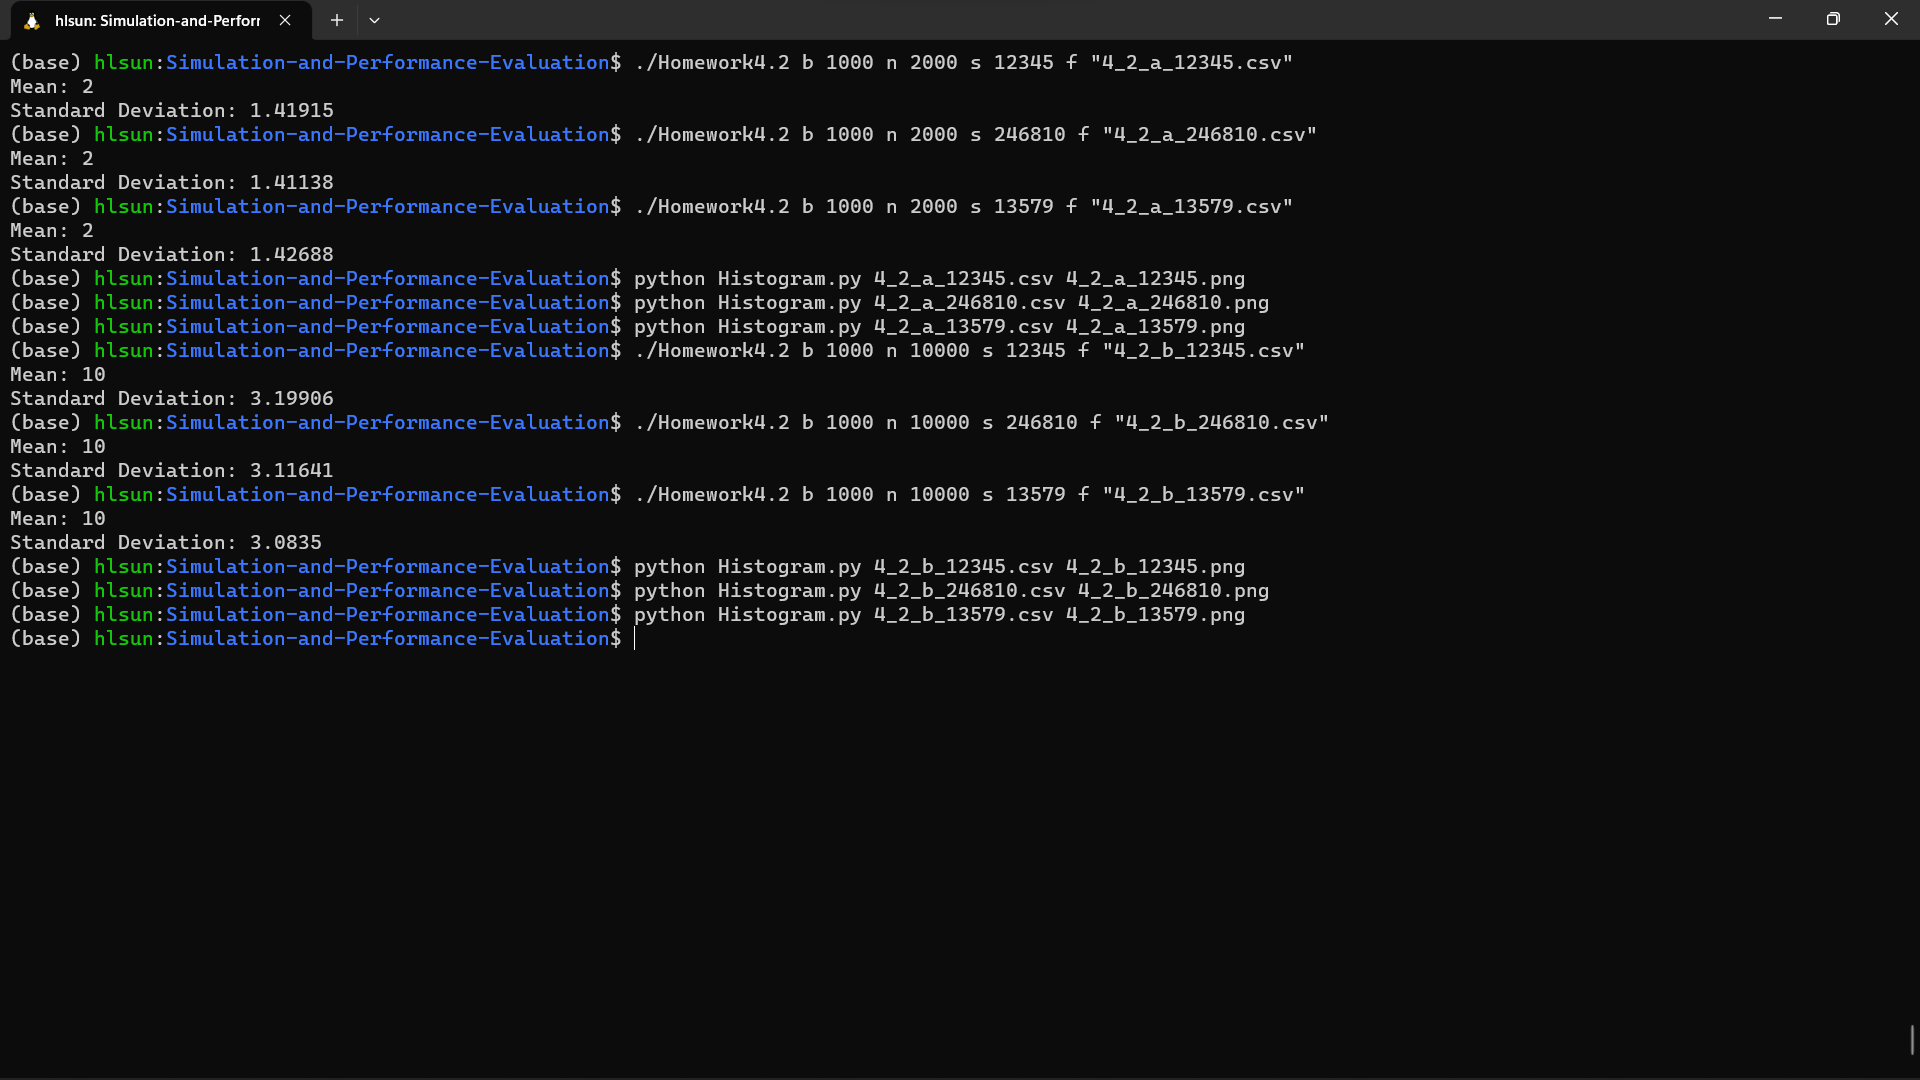
\includegraphics[scale=0.45]{Sections/Q2/4_2_terminal.png}\\
\newpage
\noindent Part A:\\\\
Seed: 12345\\
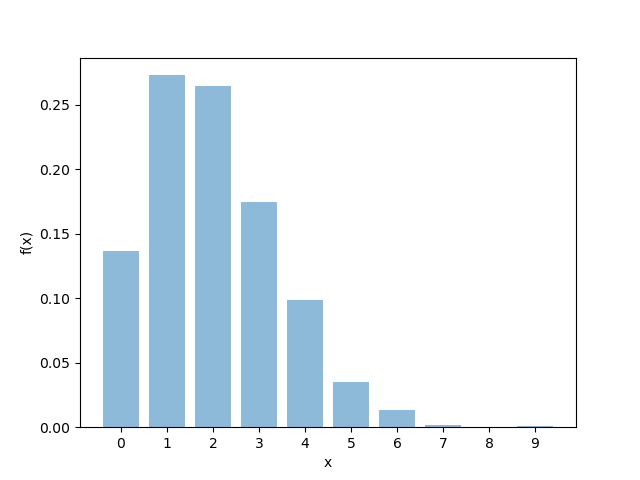
\includegraphics[scale=1]{Sections/Q2/4_2_a_12345.png}\\
\newpage
Seed: 13579\\
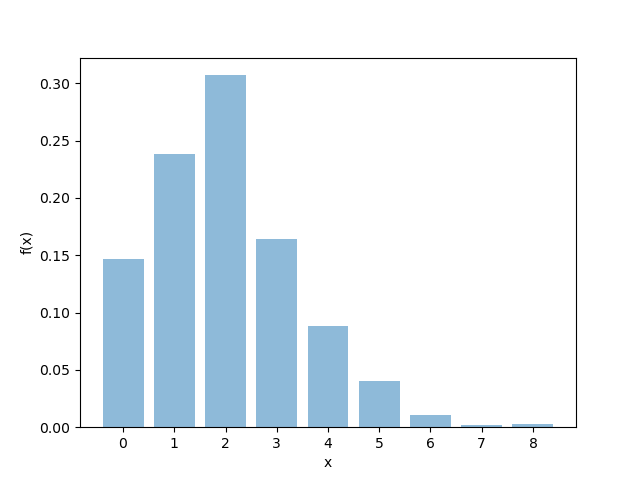
\includegraphics[scale=1]{Sections/Q2/4_2_a_13579.png}\\
\newpage
Seed: 246810\\
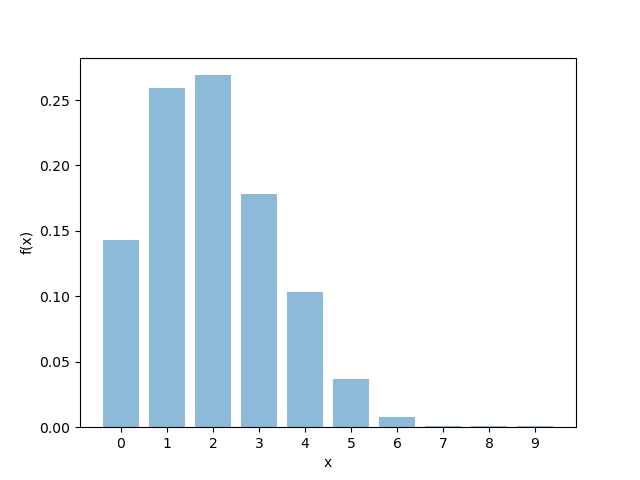
\includegraphics[scale=1]{Sections/Q2/4_2_a_246810.png}\\
\newpage
\noindent Part B:\\\\
Seed: 12345\\
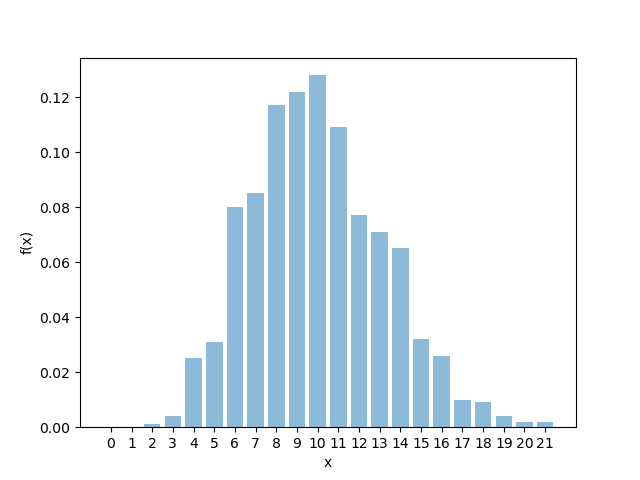
\includegraphics[scale=1]{Sections/Q2/4_2_b_12345.png}\\
\newpage
Seed: 13579\\
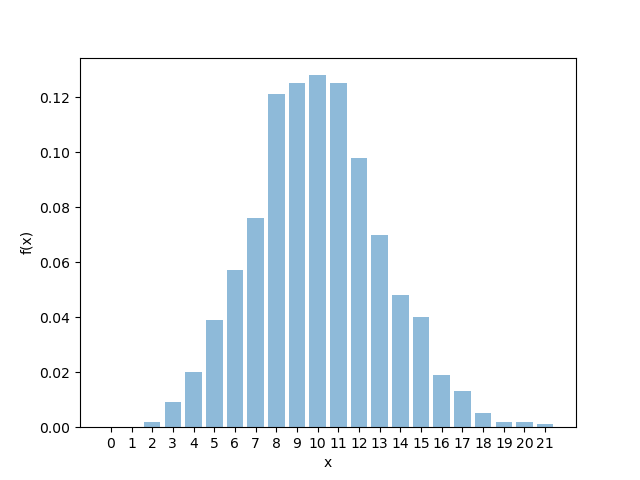
\includegraphics[scale=1]{Sections/Q2/4_2_b_13579.png}\\
\newpage
Seed: 246810\\
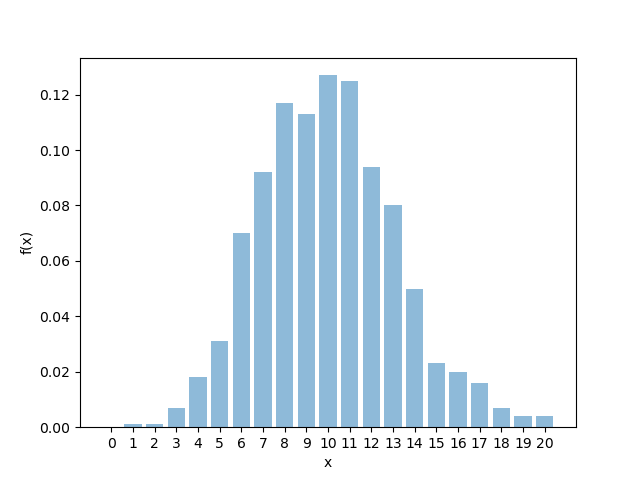
\includegraphics[scale=1]{Sections/Q2/4_2_b_246810.png}\\
\newpage

\begin{lstlisting}[style=CStyle]
/**
 * Harrison Sun (sun.har@northeastern.edu)
 * EECE 5643 - Simulation and Performance Evaluation
 * Homework 4.2
 */

#include <cstdlib>
#include <cstring>
#include <fstream>
#include <stdio.h>
#include <exception>
#include <iostream>
#include <list>
#include <math.h> 
#include <string>
#include <vector>
#include "c_lib/rvgs.h"
#include "c_lib/rngs.h"
#include "checkarg/checkarg.h"

#define DEFAULT_N_BOX		1000
#define DEFAULT_N_BALLS		2000
#define DEFAULT_SEED		12345
#define DEFAULT_OFILE		"output.txt"

/**
 * int main() - The main function
 * 
 * @param int argc - the number of arguments
 * @param char* argv[] - the arguments
 * 
 * @return 0 if the program runs successfully
 */

int main(int argc, char* argv[])
{
	// Variable Declarations
	int nBoxes{};
	int nBalls{};
	std::string outputFileName{};
	
	// doubly linked list <box number, number of balls in box>
	std::list<std::pair<long, long>> boxCount;
	
    // Set the seed
    for (int i = 0; i < argc; ++i)
    {
        if (*argv[i] == 's' && checkArg(argv[i + 1]))
        {
            PutSeed(std::stol(argv[i + 1]));
            break;
        }
        else
        {
            PutSeed(DEFAULT_SEED);
        }
    }

	// Set the number of boxes
	for (int i = 0; i < argc; ++i)
	{
		if (*argv[i] == 'b' && checkArg(argv[i + 1]))
		{
			nBoxes = std::stol(argv[i + 1]);
			break;
		}
		else
		{
			nBoxes = DEFAULT_N_BOX;
		}
	}

	// Set the number of balls
	for (int i = 0; i < argc; ++i)
	{
		if (*argv[i] == 'n' && checkArg(argv[i + 1]))
		{
			nBalls = std::stol(argv[i + 1]);
			break;
		}
		else
		{
			nBalls = DEFAULT_N_BALLS;
		}
	}

	// Set the filestream
	for (int i = 0; i < argc; ++i)
	{
		if (*argv[i] == 'f')
		{
			outputFileName = argv[i + 1];
			break;
		}
		else
		{
			outputFileName = DEFAULT_OFILE;
		}
	}

	/* Generate balls and determine which box they go in. */
	for (int i = 0; i < nBalls; ++i)
	{
		// Equilikely distribution between box 0 and box nBoxes - 1
		int box = Equilikely(0, nBoxes - 1);
		
		// Iterate through the linked list looking for the box number. If it is found, increment the count.
		// If the box is not in the list, add it to the list and set the count to 1.
		// The box is sorted in ascending order.
		bool found = false;
		for (auto it = boxCount.begin(); it != boxCount.end(); ++it)
		{
			// The box is in the list
			if (it->first == box)
			{
				it->second++;
				found = true;
				break;
			}

			// The box is not in the list and a greater box value is found
			else if (it->first > box)
			{
				boxCount.insert(it, std::make_pair(box, 1));
				found = true;
				break;
			}
		}
		
		// The box is not in the list and is greater than all boxes currently in the list
		if (!found)
		{
			boxCount.push_back(std::make_pair(box, 1));
		}
	}

	// Traverse the linked list nBalls times and determine how many boxes contain n number of balls.
	std::vector<long> boxCountVector;
	for (int i = 0; i < nBalls; ++i)
	{
		long count = 0;
		for (auto it = boxCount.begin(); it != boxCount.end(); ++it)
		{
			if (it->second == i)
			{
				count++;
			}
		}
		boxCountVector.push_back(count);
	}

	// Remove trailing zeros
	for (auto iter = boxCountVector.end() - 1; iter != boxCountVector.begin(); --iter)
	{
		if (*iter == 0)
		{
			boxCountVector.pop_back();
		}
		else
		{
			break;
		}
	}

	// Set the number of boxes with zero balls to nBoxes subtracted by the sum of the number of boxes that have balls in them
	long sum{ 0 };
	for (auto iter = boxCountVector.begin(); iter != boxCountVector.end(); ++iter)
	{
		sum += *iter;
	}
	boxCountVector.at(0) =  (nBoxes - sum);

	// Store boxCountVector as a csv file for plotting in Python
	std::ofstream outputFile;
	outputFile.open(outputFileName);
	long boxNum{ 0 };
	for (auto iter = boxCountVector.begin(); iter != boxCountVector.end(); ++iter)
	{
		// Output the probability of a box containing n number of balls
		outputFile << boxNum++ << ", " << (double)  *iter / nBoxes << std::endl;
	}
	outputFile.close();

	// Calculate the mean and standard deviation
	double mean{ 0 };
	double stdDev{ 0 };
	boxNum = 0;
	
	for (auto iter = boxCountVector.begin(); iter != boxCountVector.end(); ++iter)
	{
		mean += (double) * iter * boxNum / nBoxes;
		++boxNum;
	}

	boxNum = 0;
	
	for (auto iter = boxCountVector.begin(); iter != boxCountVector.end(); ++iter)
	{
		stdDev += (double) * iter * pow((boxNum - mean), 2);
		++boxNum;
	}

	stdDev = sqrt(stdDev / nBoxes);

	std::cout << "Mean: " << mean << std::endl;
	std::cout << "Standard Deviation: " << stdDev << std::endl;
	
	return 0;
}
\end{lstlisting}